%---------------------------------------------------------------------------%
%-                                                                         -%
%-                           LaTeX Template                                -%
%-                                                                         -%
%---------------------------------------------------------------------------%
%- Copyright (C) Huangrui Mo <huangrui.mo@gmail.com> 
%- This is free software: you can redistribute it and/or modify it
%- under the terms of the GNU General Public License as published by
%- the Free Software Foundation, either version 3 of the License, or
%- (at your option) any later version.
%---------------------------------------------------------------------------%
%->> Document class declaration
%---------------------------------------------------------------------------%
\documentclass[singlesided]{Style/uwaterloothesis}%
%- Multiple optional arguments:
%- [<singlesided|doublesided|printcopy>]% set one or two sided eprint or print
%- [draftversion]% show draft version information
%- [standard options for book class: draft|paper size|font size|...]%
%---------------------------------------------------------------------------%
%->> Document settings
%---------------------------------------------------------------------------%
\usepackage[myhdr,list]{Style/artratex}% document settings
%- usage: \usepackage[option1,option2,...,optionN]{artratex}
%- Multiple optional arguments:
%- [bibtex|biber]% set bibliography processor and package
%- [<numbers|super|authoryear|alpha>]% set citation and reference style
%- <numbers>: textual: Jones [1]; parenthetical: [1]
%- <super>: textual: Jones superscript [1]; parenthetical: superscript [1]
%- <authoryear>: textual: Jones (1995); parenthetical: (Jones, 1995)
%- <alpha>: textual: not available; parenthetical: [Jon95]
%- [geometry]% reconfigure page layout via geometry package
%- [lscape]% provide landscape layout environment
%- [myhdr]% enable header and footer via fancyhdr package
%- [color]% provide color support via xcolor package
%- [background]% enable page background
%- [tikz]% provide complex diagrams via tikz package
%- [table]% provide complex tables via ctable package
%- [list]% provide enhanced list environments for algorithm and coding
%- [math]% enable some extra math packages
\usepackage{Style/artracom}% user defined commands
%---------------------------------------------------------------------------%
%->> Document inclusion
%---------------------------------------------------------------------------%
%\includeonly{Tex/Chap_1,...,Tex/Chap_N}% selected files compilation
%---------------------------------------------------------------------------%
%->> Document content
%---------------------------------------------------------------------------%
\begin{document}
%-
%-> Frontmatter: title page, abstract, content list, symbol list, preface
%-
\frontmatter% initialize the environment
%---------------------------------------------------------------------------%
%->> Titlepage information
%---------------------------------------------------------------------------%
%-
%-> Title info
%-
\title[\LaTeX{} Thesis Template of UW]{\LaTeX{} Thesis Template\\ of\\ The University of Waterloo}% \title[short title for headers]{Long title of thesis}
\author{Huangrui Mo}
\degree{Doctor of Philosophy}
\discipline{Mechanical Engineering}
\maketitle
%-
%-> Examining Committee Membership
%-
\intotoc{Examining Committee Membership}% add a corresponding item to the contents table and bookmark
\begin{committee}
    \noindent
    The following served on the Examining Committee for this thesis. The decision of the Examining Committee is by majority vote.

    \begin{center}
        %\footnotesize% fontsize
        \setlength{\tabcolsep}{10pt}% column separation
        \renewcommand{\arraystretch}{3}% row space 
        \begin{tabular}{lc}
            External Examiner & \parbox[t]{10cm}{Dr. Luc Bauwens\\Professor, Mechanical and Manufacturing Engineering\\University of 
Calgary}\\
            Supervisors & \parbox[t]{10cm}{Dr. Fue-Sang Lien\\Professor, Mechanical and Mechatronics Engineering\\University of Waterloo}\\
             & \parbox[t]{10cm}{Dr. Fan Zhang\\Senior Scientist, Advanced Energetics Group\\Defence Research and Development Canada}\\
             & \parbox[t]{10cm}{Dr. Duane Cronin\\Professor, Mechanical and Mechatronics Engineering\\University of Waterloo}\\
            Internal Members & \parbox[t]{10cm}{Dr. Cecile Devaud\\Professor, Mechanical and Mechatronics Engineering\\University of Waterloo}\\
             & \parbox[t]{10cm}{Dr. Jean-Pierre Hickey\\Professor, Mechanical and Mechatronics Engineering\\University of Waterloo}\\
            Internal-External Member & \parbox[t]{10cm}{Dr. Lilia Krivodonova\\Professor, Applied Mathematics\\University of Waterloo}\\
        \end{tabular}
    \end{center}
\end{committee}
%-
%-> Author's declaration
%-
\intotoc{Author's Declaration}% add a corresponding item to the contents table and bookmark
\begin{declaration}
    \noindent
    I hereby declare that I am the sole author of this thesis. This is a true copy of the thesis, including any required final revisions, as accepted by my examiners.

    \bigskip

    \noindent
    I understand that my thesis may be made electronically available to the public.
\end{declaration}
%-
%-> Statement of Contributions
%-
%\intotoc{Statement of Contributions}% add a corresponding item to the contents table and bookmark
%\begin{contribute}
%\end{contribute}
%-
%-> Permissions
%-
%\intotoc{Permissions}% add a corresponding item to the contents table and bookmark
%\begin{permission}
%    \noindent
%\end{permission}
%-
%-> Abstract
%-
\intotoc{Abstract}% add a corresponding item to the contents table and bookmark
\begin{abstract}
    This is a short brochure on how to write your thesis by using this \LaTeX{} template. It's easy, efficient and straightforward. What you need to do, no matter you are familiar with \LaTeX{} or not, is to have a try.
\end{abstract}
%-
%-> Acknowledgements
%-
\intotoc{Acknowledgements}% add a corresponding item to the contents table and bookmark
\begin{acknowledgements}

    I owe my deepest gratitude and appreciation to my doctoral advisors: Dr. Fue-Sang Lien, Dr. Fan Zhang, and Dr. Duane Cronin. Dr. Fue-Sang Lien has always been supportive, approachable, and helpful throughout my doctoral study. His encouragement and understanding helped me go though the difficulties and created the space for me to develop research ideas. Working with Dr. Fan Zhang has been the most amazing experience in my life. I have been always fascinated by his insights on physics and the ability to instantly and accurately identify the key problems based on a set of fragmented information. His keen and open-minded guidance inspired my interests in the field of my doctoral study, shaped my critical thinking, and challenged me to be a higher level thinker. It was an enlightening and enriching experience to collaborate with Dr. Duane Cronin. Whenever I needed advice, he was ready and patient to help. He was always kind to teach me and willing to share his experience and vision on how to be a professional, rigorous, and persuasive researcher. The moments I interacted with and the knowledge I learned from my outstanding advisors will be remembered by me throughout the rest of my life.

    I am grateful to Natural Sciences and Engineering Research Council of Canada (NSERC), Defence Research and Development Canada (DRDC), and Waterloo CFD Engineering Consulting Inc (WATCFD) for the financial support of this research project. This work was made possible by the facilities of the Shared Hierarchical Academic Research Computing Network (SHARCNET: www.sharcnet.ca) and Compute/Calcul Canada.

    I would like to thank the official members of my examining committee for their efforts in reviewing my thesis and providing helpful suggestions. In addition, I want to express my gratitude to Dr. Jean-Pierre Hickey for his kind help with my teaching practice, to Dr. Cecile Devaud for her helpful comments on my comprehensive examination report, to Dr. Lilia Krivodonova for her thoughtful teaching on numerical solutions of partial differential equations, and to Dr. Luc Bauwens for taking his time to come and attend my examination in person. I also want to thank my colleagues in the Energy Research Center for their support and discussions and the faculty and staff in the Mechanical and Mechatronics Engineering department for their assistance and help throughout my doctoral study. Finally, I am indebted to my family for their continuous support and understanding with my pursuit of scientific research.

\end{acknowledgements}
%-
%-> Dedication
%-
%\intotoc{Dedication}% add a corresponding item to the contents table and bookmark
%\begin{dedication}
%    Dedication (included if necessary)
%\end{dedication}
%---------------------------------------------------------------------------%
% title page, abstract, dedication
{% content list region
\linespread{1.1}% local line space
\intotoc*{\cleardoublepage}{\contentsname}% add link to bookmark
\tableofcontents% content catalog
\intotoc*{\cleardoublepage}{\listfigurename}% add link to bookmark
\listoffigures% figure catalog
\intotoc*{\cleardoublepage}{\listtablename}% add link to bookmark
\listoftables% table catalog
}
%%
%% >>> Nomenclatures
%%
\chapter{Nomenclature}

\section*{Roman Characters}
\nomenclatureitem[\textbf{Unit}]{\textbf{Symbol}}{\textbf{Description}}
\nomenclatureitem{\textrm{a}}{empirical stoichiometric coefficient}
\nomenclatureitem[$m/s$]{\textrm{c}}{frozon sound speed}

\section*{Greek Characters}
\nomenclatureitem{\textbf{Symbol}}{\textbf{Description}}
\nomenclatureitem{$\alpha$}{velocity transmission factor}
\nomenclatureitem{$\beta$}{temperature transmission factor}

\section*{Subscripts}
\nomenclatureitem{\textbf{Symbol}}{\textbf{Description}}
\nomenclatureitem{$CJ$}{Chapman-Jouguet state}
\nomenclatureitem{$c$}{convection}

\section*{Operators}
\nomenclatureitem{\textbf{Symbol}}{\textbf{Description}}
\nomenclatureitem{$\triangledown$}{difference}
\nomenclatureitem{$\nabla$}{gradient operator}

\section*{Abbreviations}
\nomenclatureitem{\textbf{Acronym}}{\textbf{Description}}
\nomenclatureitem{CJ}{Chapman-Jouguet}
\nomenclatureitem{ZND}{Zel'dovich-von Neumann-Doering}

% list of symbols, preface content
%-
%-> Mainmatter
%-
\mainmatter% initialize the environment
%---------------------------------------------------------------------------%
%->> Main content
%---------------------------------------------------------------------------%
\chapter{A Brief Guide}
\label{chap:guide}

\section{What is \LaTeX{}} % (fold)

\LaTeX{} (pronounced "Lah-tech" or "Lay-tech") is a macro package created by Leslie Lamport based on \TeX{}. As a document preparation system for high-quality typesetting in almost any forms of publishing, \LaTeX{} is not the name of a particular editing program, but refers to the encoding or tagging conventions that are used in \LaTeX{} documents \citep{website:wikipedia,website:latex}.

% section What is \LaTeX{} (end)

\section{Why use \LaTeX?}

There are a lot of good reasons why you need to use \LaTeX{}, the most significant one is the following:
\begin{itemize}
    \item Allows you to clearly separate the content from the format of your document.
    \item Let you concentrate on your ideas, not visual appearance.
\end{itemize}

You can concentrate purely on the structure and contents of your document, not superficial layout issues. You don't need to manually adjust fonts, text sizes, line heights, or text flow for readability, as \LaTeX{} takes care of them automatically. \citep{website:wikibook}
\begin{figure}[!htbp]
    \centering
    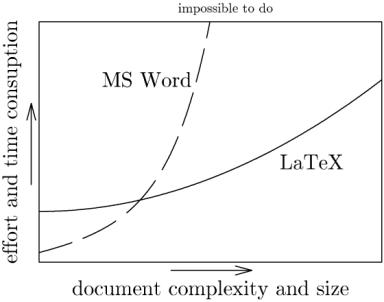
\includegraphics[width=0.6\textwidth]{compare}
    \caption{Comparison between Microsoft Word and \LaTeX{} [From Google Images]}
    \label{fig:compare}
\end{figure}

\section{How to use?} % (fold)

\subsection{Installation} % (fold)
LaTeX is based on open-source code, so it is available on most computing platforms as free software.
\begin{itemize}
    \item Linux: TeXLive distribution. 
    \item MacOS: Mactex or TeXLive.
    \item Windows: MikTeX or TeXLive. 
\end{itemize}

Note: the best resource that can be used to learn \LaTeX{} is "\LaTeX{} Wikibook", which is available online.

Note: to use \LaTeX{}, you need a text editor for writing and editing ".tex" files. To open the ".tex" files in this template, you need a text editor which supports "UTF-8" encoding. Free options for different platforms are the following:
\begin{itemize}
    \item Linux: vim. 
    \item MacOS: TeXShop, Macvim.
    \item Windows: Texmaker, Gvim, Notepad++. 
\end{itemize}
% subsection Installation (end)

\subsection{Give a try} % (fold)
After downloading this template and installing a \LaTeX{} distribution. It's time to have a try:
\begin{itemize}
    \item Linux: run Compile.sh
    \item MacOS: run Compile.sh
    \item Windows: run Compile.bat
\end{itemize}

Note: It's recommended to use the provided scripts to compile your \LaTeX{} files. It will automatically search and include files without explicitly specifying relative paths. If you do not use them for compilation, you need to specify the relative path in each "\verb+\input{ }+" command, or the \LaTeX{} will complain that it can not find some files.

Note: the bash script "Compile.sh" hasn't been tested on MacOS. If there are some errors, please give me your feedback, thank you so much.

% subsection Give a try (end)

\subsection{Include math} % (fold)
\LaTeX{} realization of Equation~\ref{eq:N-S_equation} is something like this:
\begin{center}
    \small
    \begin{verbatim}
    \begin{equationa}\label{eq:N-S_equation}
        \frac{\partial (\rho\mathbf{v})}{\partial t} +
        \nabla \cdot (\rho \mathbf{v} \mathbf{v}) =
        -\nabla p + \nabla \cdot\mathbf{T} + \mathbf{f}. 
    \end{equation}    
\end{verbatim}
\end{center}

\begin{equation}\label{eq:N-S_equation}
    \frac{\partial (\rho\mathbf{v})}{\partial t} + \nabla \cdot (\rho \mathbf{v} \mathbf{v}) = -\nabla p + \nabla \cdot\mathbf{T} + \mathbf{f}. 
\end{equation}    
% subsection Include math (end)

\subsection{Include Graphics} % (fold)
Note: inluding figures may seem to be scary by looking at the codes. However, the fact is that you only need to modify the names in each part, the rest are simply copy and paste. These codes are all available in the file "Useful Commands.txt".

Figure~\ref{fig:ITC_Q_Criteria} is an example for including a single figure.
\begin{center}
    \small
    \begin{verbatim}
        \begin{figure}[!htbp]
            \centering
            \includegraphics[width=\MyFactor\textwidth]{ITC_Q_Criteria}
            \caption{An Example for including a single figure}
            \label{fig:ITC_Q_Criteria}
        \end{figure}
    \end{verbatim}
\end{center}

Figure~\ref{fig:HC_OASPL} is an example for including multiple figuress. 
\begin{figure}[!htbp]
    \centering
    \includegraphics[width=\MyFactor\textwidth]{ITC_Q_Criteria}
    \caption{An Example for including a single graph}
    \label{fig:ITC_Q_Criteria}
\end{figure}
\begin{center}
    \small
    \begin{verbatim}
        \begin{figure}[!htbp]
            \centering
            \begin{subfigure}[b]{\MySubFactor\textwidth}
                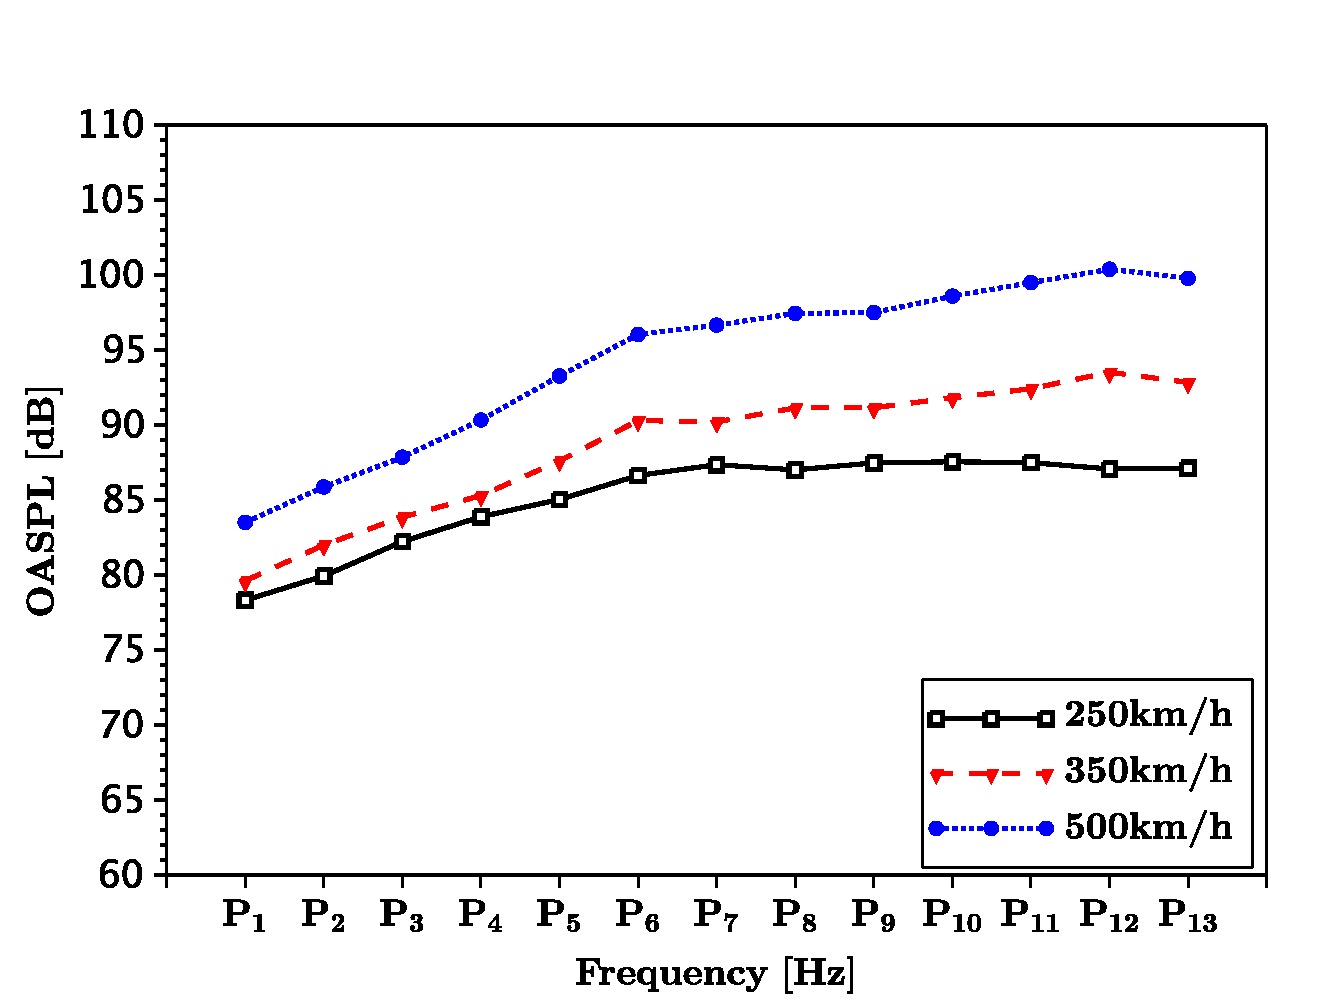
\includegraphics[width=\textwidth]{HC_OASPL_A}
                \caption{}
                \label{fig:HC_OASPL_A}
            \end{subfigure}%
            ~% add a small space
            \begin{subfigure}[b]{\MySubFactor\textwidth}
                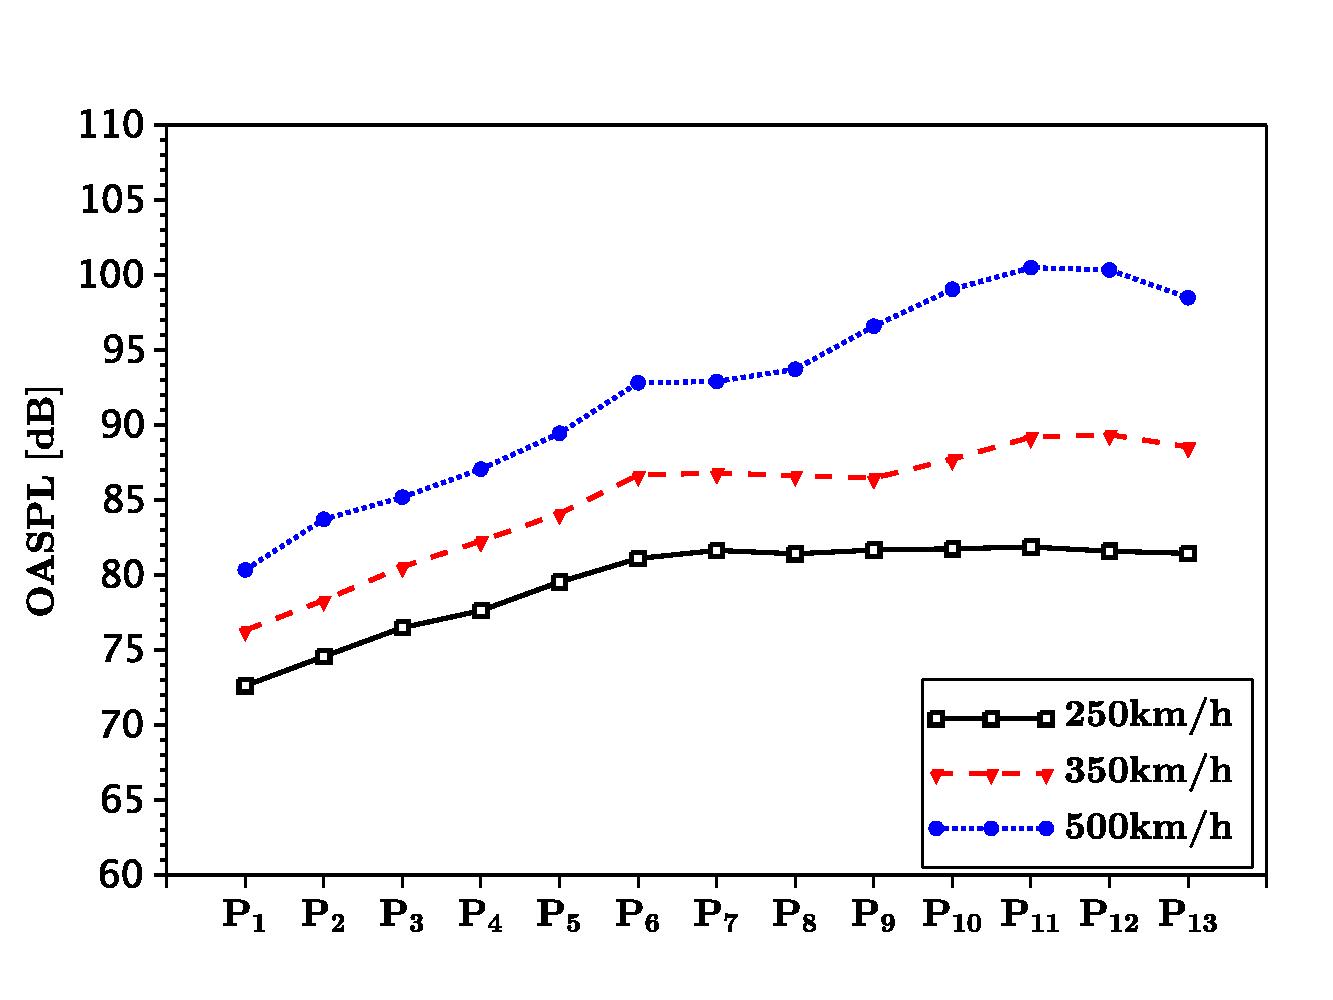
\includegraphics[width=\textwidth]{HC_OASPL_B}
                \caption{}
                \label{fig:HC_OASPL_B}
            \end{subfigure}%
            \\% change line
            \begin{subfigure}[b]{\MySubFactor\textwidth}
                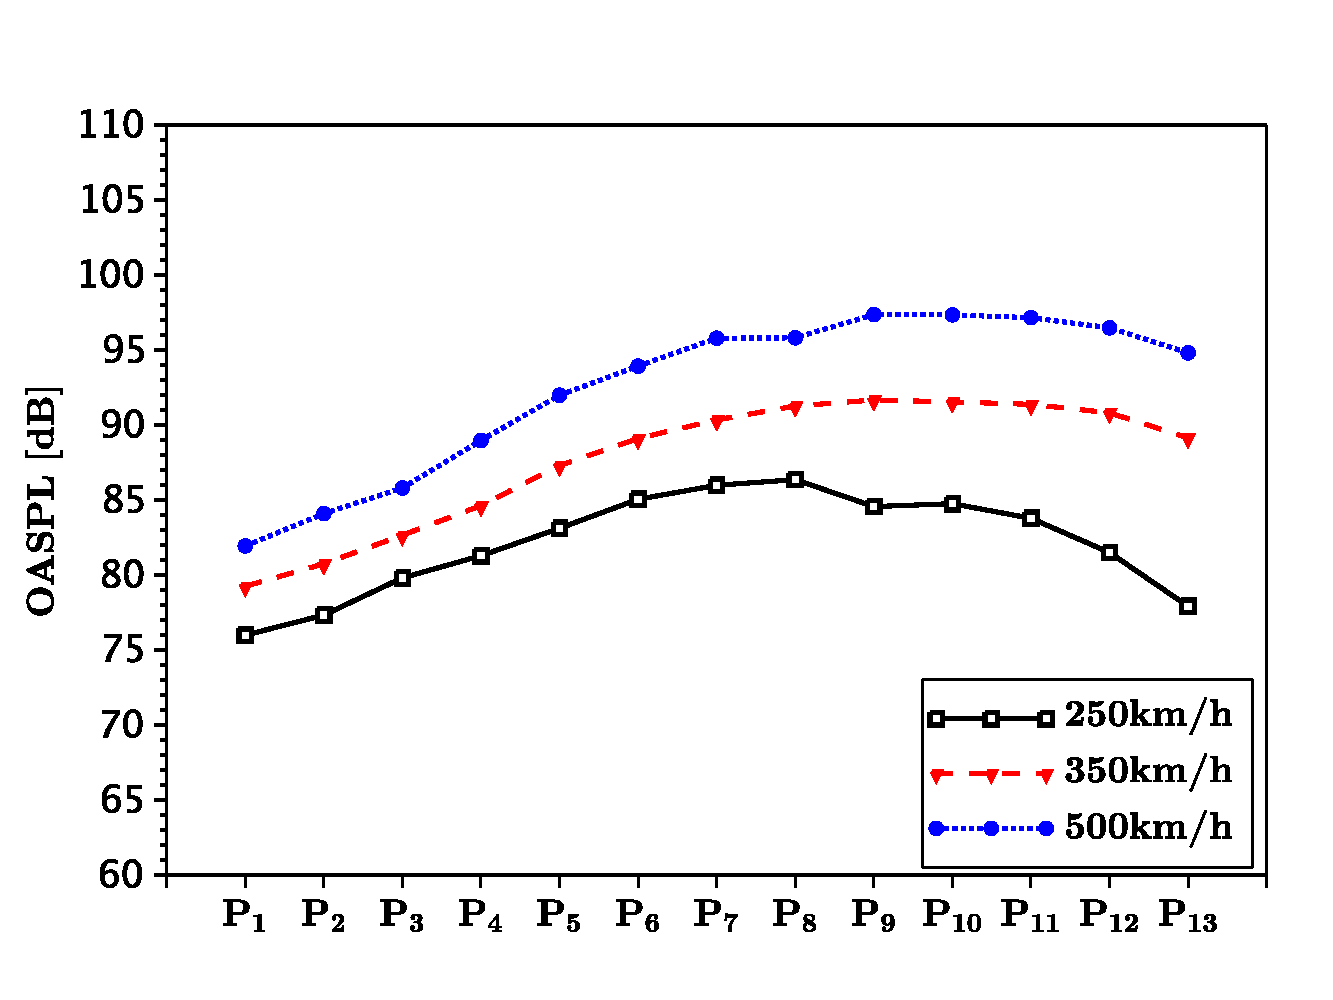
\includegraphics[width=\textwidth]{HC_OASPL_C}
                \caption{}
                \label{fig:HC_OASPL_C}
            \end{subfigure}%
            ~% add a small space
            \begin{subfigure}[b]{\MySubFactor\textwidth}
                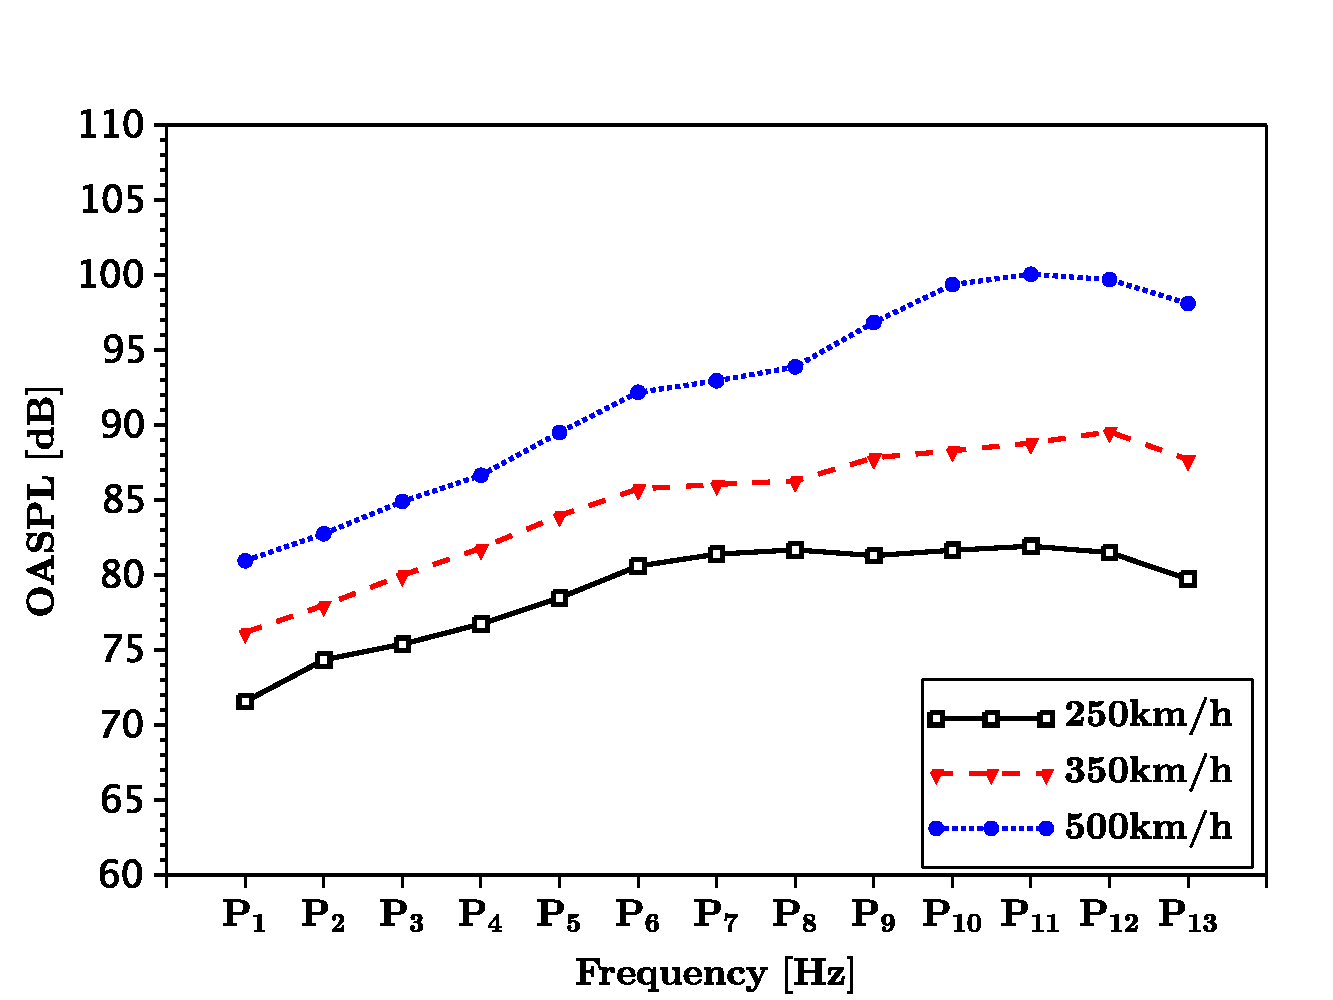
\includegraphics[width=\textwidth]{HC_OASPL_D}
                \caption{}
                \label{fig:HC_OASPL_D}
            \end{subfigure}%
            \caption{An Example for including multiple figures}
            \label{fig:HC_OASPL}
        \end{figure}
    \end{verbatim}
\end{center}
\begin{figure}[!htbp]
    \centering
    \begin{subfigure}[b]{\MySubFactor\textwidth}
        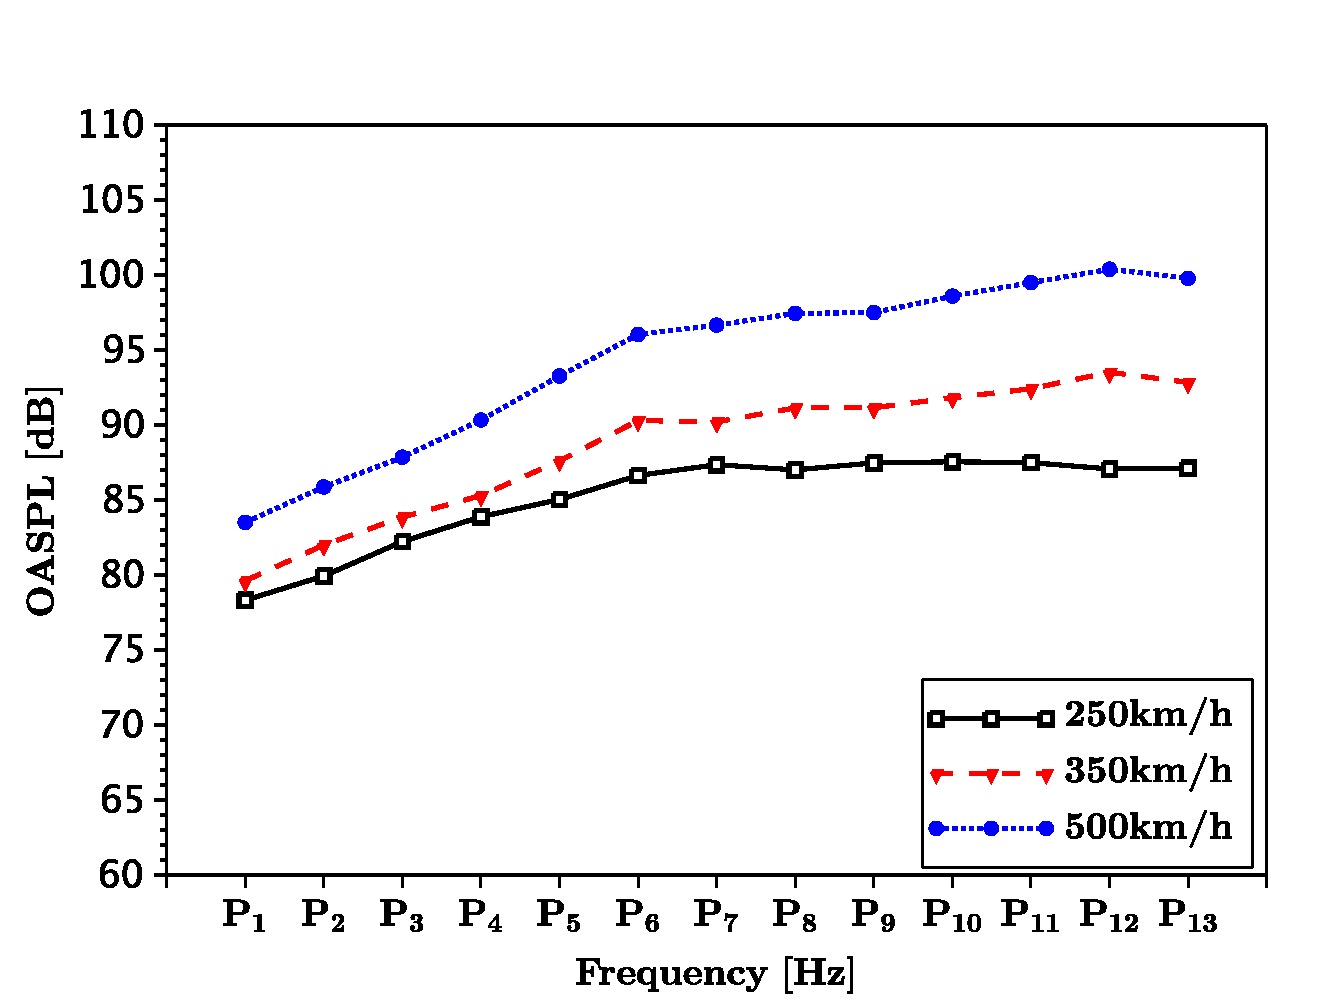
\includegraphics[width=\textwidth]{HC_OASPL_A}
        \caption{}
        \label{fig:HC_OASPL_A}
    \end{subfigure}%
    ~% add a small space
    \begin{subfigure}[b]{\MySubFactor\textwidth}
        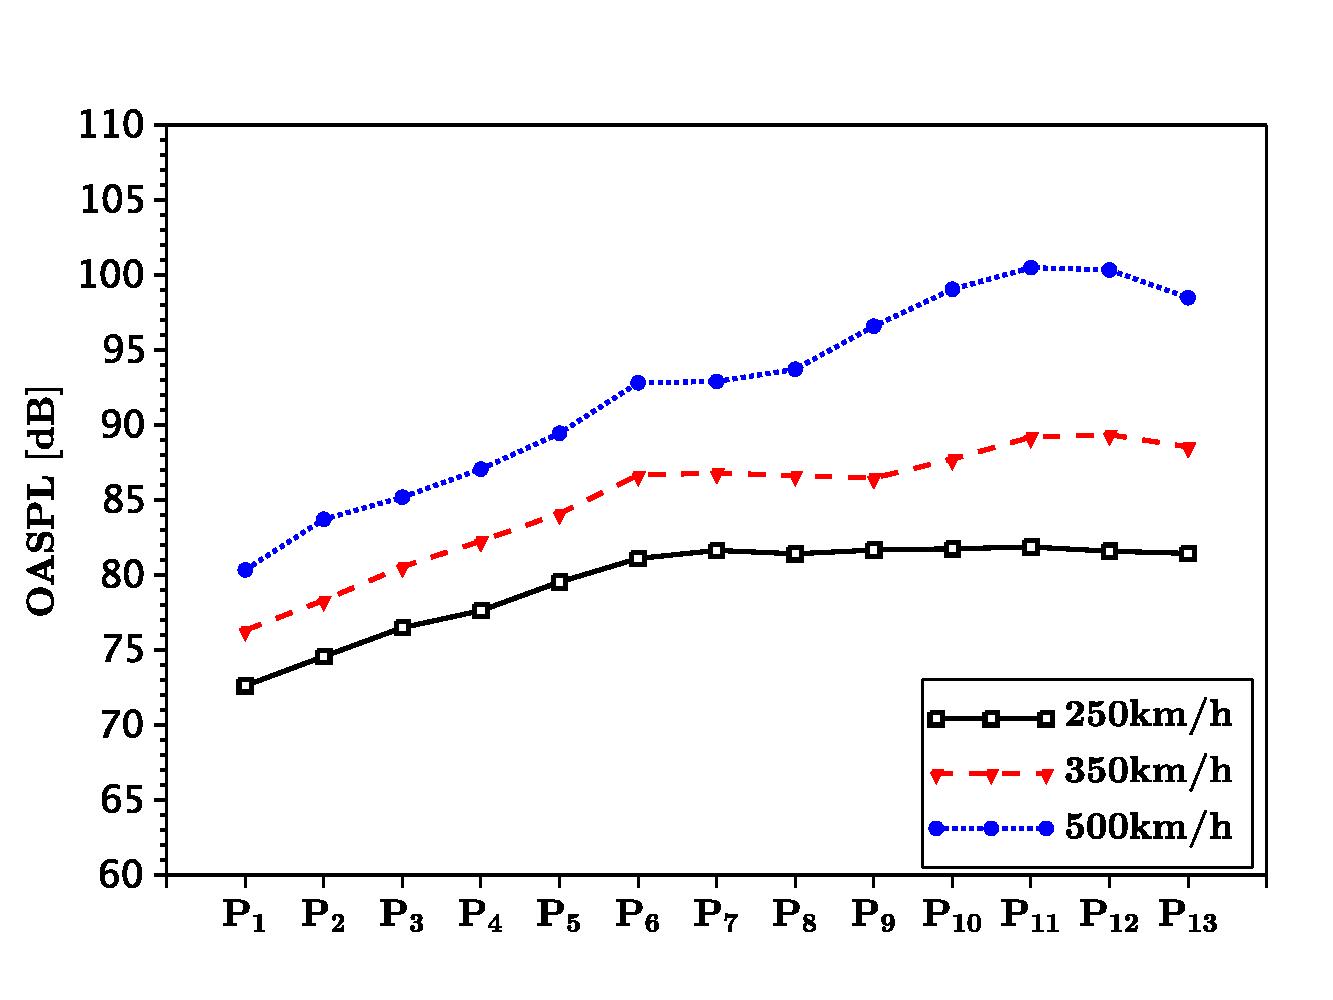
\includegraphics[width=\textwidth]{HC_OASPL_B}
        \caption{}
        \label{fig:HC_OASPL_B}
    \end{subfigure}%
    \\% change line
    \begin{subfigure}[b]{\MySubFactor\textwidth}
        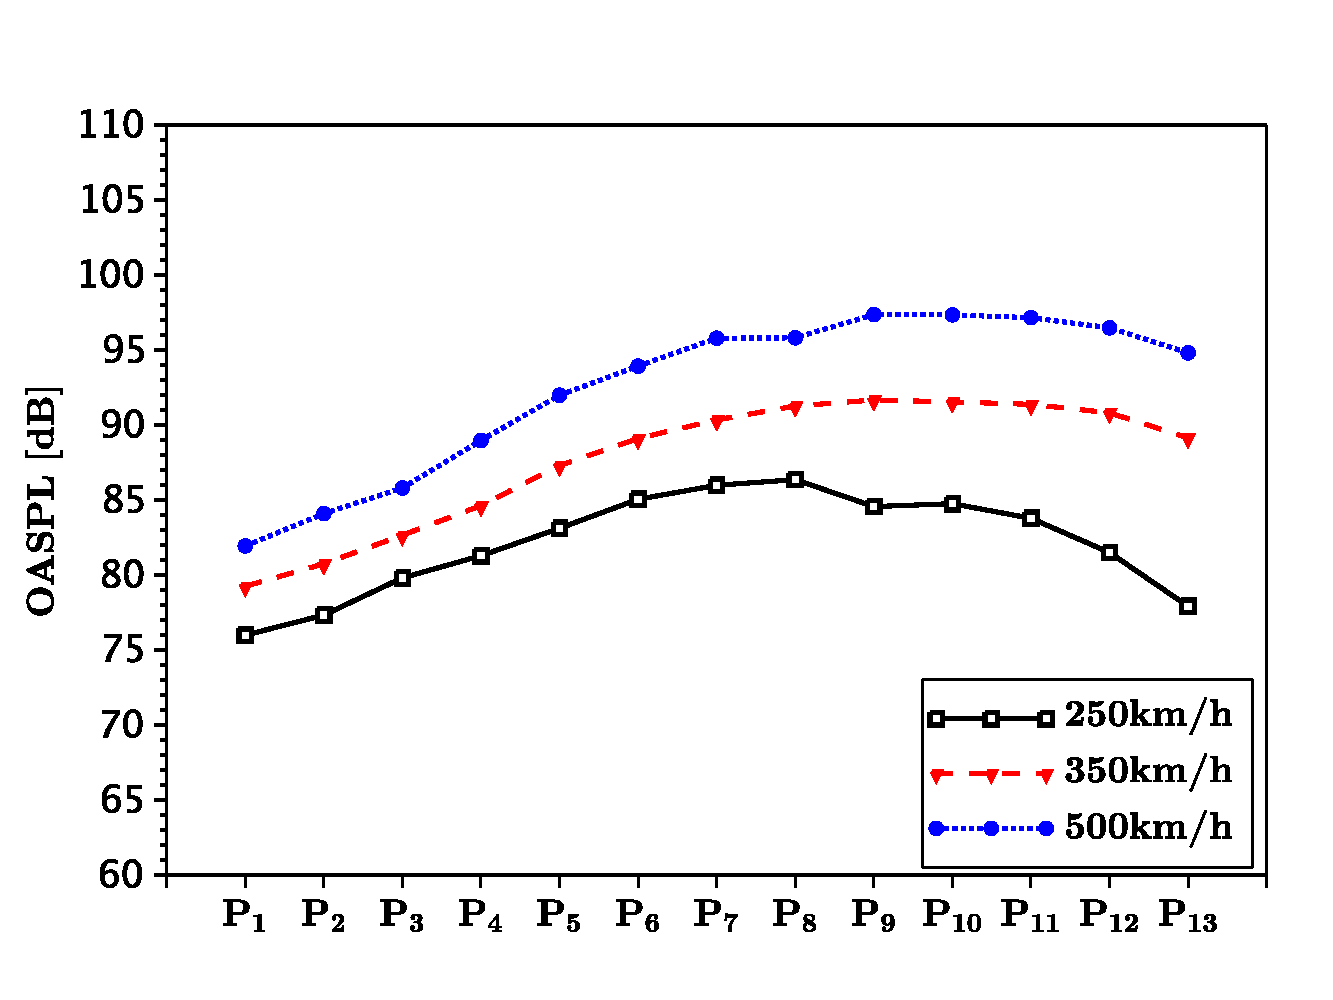
\includegraphics[width=\textwidth]{HC_OASPL_C}
        \caption{}
        \label{fig:HC_OASPL_C}
    \end{subfigure}%
    ~% add a small space
    \begin{subfigure}[b]{\MySubFactor\textwidth}
        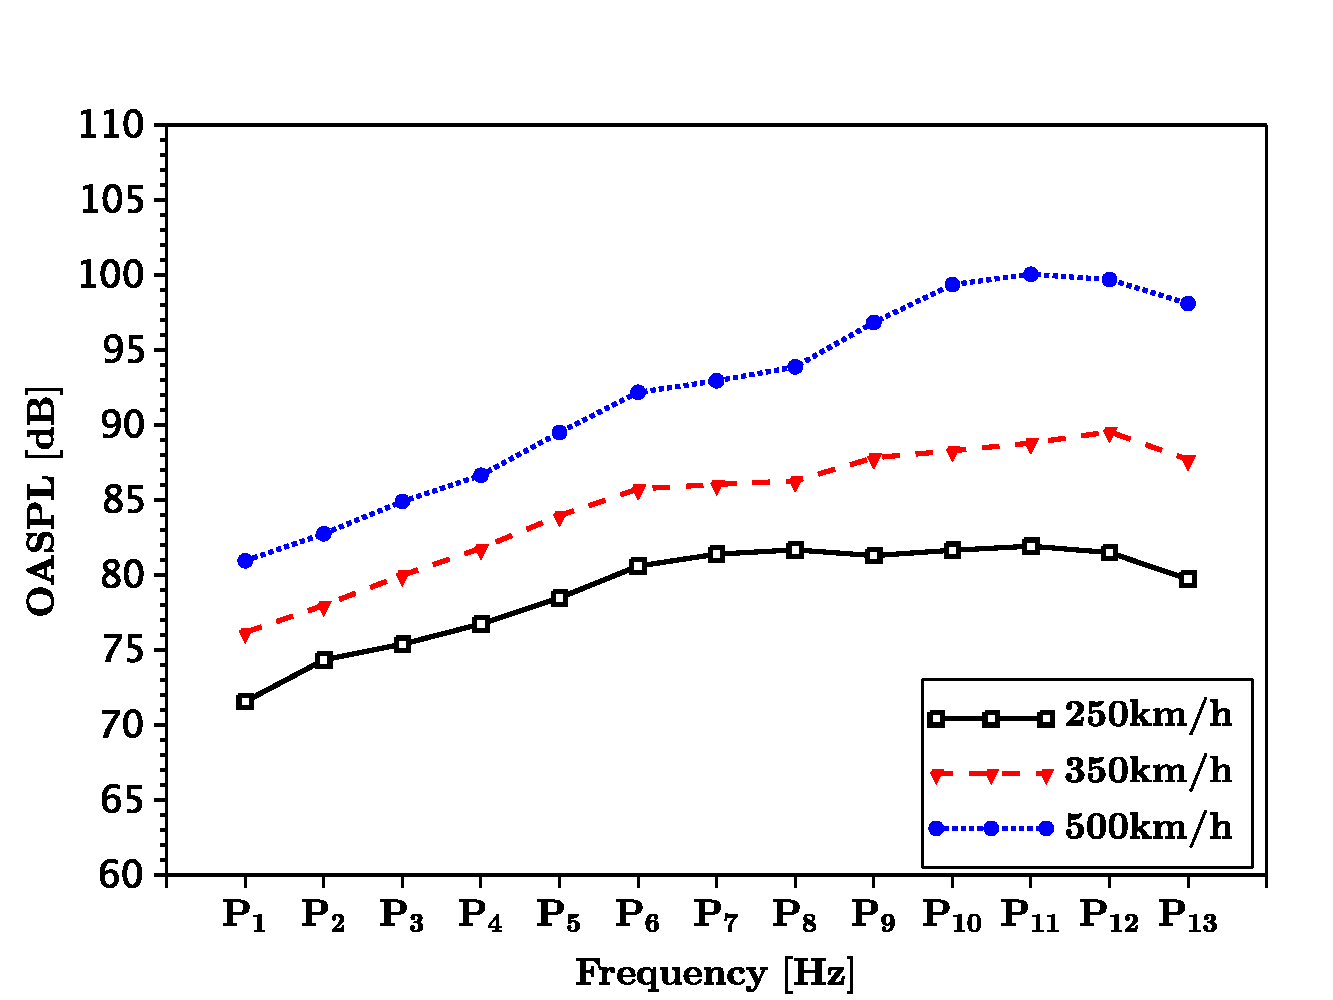
\includegraphics[width=\textwidth]{HC_OASPL_D}
        \caption{}
        \label{fig:HC_OASPL_D}
    \end{subfigure}%
    \caption{An Example for including multiple figures}
    \label{fig:HC_OASPL}
\end{figure}
% subsection Include Graphics (end)

\subsection{Include a citation} % (fold)
Suppose you are going to cite an article named "Document Preparation System", the procedures are:
\begin{itemize}
    \item Use Google Scholar search "Document Preparation System".
    \item Open "Cite" and choose "Import to Bibtex" under the target item.
    \item Copy the citation information of this article into the file "Myrefs.bib"
    \item Research dominant: cite this article by \verb+\citep{lamport1986document}+ like here \citep{lamport1986document}
    \item Citation dominant: cite this article by \verb+\citet{lamport1986document}+ like here \citet{lamport1986document}
    \item References list is generated automatically.
\end{itemize}
% subsection Include a citation (end)
\subsection{Generate nomenclature} % (fold)
In this template, a simple command for adding nomenclatures is provided. Therefore, packages for automatical nomenclature generation are not included. From my point of view, there is no need to use those packages and make things complicated. However, if you insist, there are a lot of available packages for creating nomenclatures. Recommended options are (Please Google the one you want to know):
\begin{itemize}
    \item listofsymbols
    \item nomencl
\end{itemize}
% subsection Generate nomenclature automatically (end)
% section How to use? (end)

\section{File Tree of Current Template} % (fold)
\begin{itemize}
    \item Thesis.tex: main tex file, which acts like the main function in C++.
    \item Style: Store template configuration files, which act like subfunctions.
    \item Tmp: Store files generated by compilation.
    \item Biblio: Store information of references.
    \item Img: Store images.
    \item Tex: Store files for your content, this is the working directory.
        \begin{itemize}
            \item Frontpages: content of front pages, like authorship, abstract, etc.
            \item Prematter: content of nomenclature, etc.
            \item Main$\_$Content: index for chapters you want to include into your current content.
            \item Chap$\_$***: your content for each chapters.
            \item Appendix: appendix.
            \item Useful Commands: collection of useful commands.
        \end{itemize}
\end{itemize}

Note: this template can be easily adapted to other writing purposes such as articles. What you need to do is to change and adjust a few items in the "Thesis.tex" file, which would be very easy after you are a little familiar with using \LaTeX{}. Like :

Change \verb+\documentclass{uwaterloothesis}+ to \verb+\documentclass{article}+
% section File Tree of Current Template (end)

Note: available options for configureing current template.
\begin{footnotesize}
\begin{verbatim}
%%%%% --------------------------------------------------------------------------------
%%
%%%%*************************Document Class Declaration*******************************
%%
\documentclass[doublesided]{uwaterloothesis}% thesis template of University of Waterloo
%% Multiple Options:
%% [doublesided] % change to double-sided style, default is single-sided
%% [printcopy] % if printed, need this for a uniform binding width
%% [draftversion] % show draft version information, default is no show
%% [standard options for book class]
%%%%% --------------------------------------------------------------------------------
%%
%%%%**************************Command Define and Settings*****************************
%%
\usepackage{commons}% common settings
%% usage: \usepackage[option1,option2,...,optionN]{commons}
%% Multiple Options:
%% [fancyhdr] % configure header and footer by fancydhr package
%% [uwaterloo] % one available header and footer style, will auto enable fancyhdr
%% [geometry] % configure page layout by geometry package
%% [numeric] % enable numeric citation mode replace the default "APA" style
%% [list] % enable enhanced list environments, useful for Algorithm and Coding
%% [color] % enable color package to use color, current package is xcolor
%% [background] % enable page background, will auto enable color package
%% [tikz] % enable tikz for complex diagrams, will auto enbale color package
%% [table] % enable a table package for complex tables, current is ctable
\usepackage{custom}% user defined commands
\end{verbatim}
\end{footnotesize}

\section{Feedback and Problems} % (fold)
Please feel free to send me emails for any related problems:
\begin{center}
huangrui.mo@uwaterloo.ca
\end{center}
% section Feedback and Problems (end)
%%%%% ++++++++++++++++++++++++++++++++++++++++++++++++++++++++++++++++++++++++++++++
%%%%% ++++++++++++++++++++++++++++++++++++++++++++++++++++++++++++++++++++++++++++++

%---------------------------------------------------------------------------%
% main content
%-
%-> Appendix
%-
\cleardoublepage%
\appendix% initialize the environment
\chapter*{APPENDICES}
\intotoc{APPENDICES}

\chapter{Other Imformation}
% appendix content
%-
%-> Backmatter: bibliography, glossary, index
%-
\backmatter% initialize the environment
\intotoc*{\cleardoublepage}{\bibname}% add link to toc
\bibliography{Biblio/ref}% bibliography
\end{document}
%---------------------------------------------------------------------------%

